\documentclass[12pt]{article}

%===============================
%
%          📦 Paquetes
%
%===============================

\usepackage[a4paper, top=2cm, bottom=2cm, left=2.5cm, right=2.5cm]{geometry}
\usepackage[spanish,es-noshorthands]{babel}
\usepackage[utf8]{inputenc}
\usepackage{amsmath}
\usepackage{amssymb}
\usepackage{multicol}
\usepackage{graphicx}
\usepackage{hyperref}
\usepackage{booktabs}
\usepackage{pgfplots}
\pgfplotsset{compat=1.18}
\usepackage[spanish]{babel}

\title{
  \vspace{2cm}
  \pagenumbering{gobble}
  
\includegraphics[width=5cm]{../../../../../assets/logo-utp.png} \\
  \vspace{1cm}
  \textbf{Universidad Tecnológica del Perú} \\
  \vspace{2cm}
  \textbf{Cálculo I} \\
  \vspace{1cm}
  \large \textbf{Taller 2}
}
\author{
  \textbf{Diaz Angeles Gary Shandé} - \texttt{U21217143} \\
  \textbf{Sanchez Leturia Jonathan} - \texttt{u20240073} \\
  \textbf{Abad Yamasaki David Antony} - \texttt{u21208456} \\
  \textbf{Torres Vara, Mateo Nicolas} - \texttt{u24308542} \\
  \textbf{Ventura Villaca Diego} - \texttt{u21216703} \\
  \texttt{Sección 26965}
}
\date{}

\begin{document}
\maketitle

\newpage
\section{Objetivo}
Adquirir una vivienda propia en un plazo de 5 a\~nos, mediante una adecuada planificaci\'on financiera.

\section{An\'alisis de la situaci\'on actual}
\begin{itemize}
	\item Ingresos mensuales del grupo/familia.
	\item Gastos fijos (alimentaci\'on, transporte, servicios, etc.).
	\item Capacidad de ahorro.
	\item Opciones de financiamiento (cr\'editos hipotecarios).
\end{itemize}

\section{Ejecuci\'on}
\begin{itemize}
	\item Buscar propiedades en plataformas digitales.
	\item Comparar precios y ubicaciones.
	\item Utilizar simuladores de cr\'edito hipotecario.
	\item Gestionar ahorros con ``bono mi vivienda''.
	\item Compra en preventa.
	\item Llevar control del presupuesto.
\end{itemize}

\section{Estrategias}
\begin{itemize}
	\item Ahorrar un porcentaje fijo mensual (ej.: 20\%).
	\item Reducir gastos innecesarios.
	\item Evaluar diferentes bancos.
	\item Definir metas de ahorro a corto, mediano y largo plazo.
\end{itemize}

\section{Cronograma}
\begin{itemize}
	\item A\~no 1--2: Ahorro inicial y an\'alisis del mercado.
	\item A\~no 3--4: Evaluaci\'on y selecci\'on de vivienda + tr\'amite de cr\'edito.
	\item A\~no 5: Inicio del pago de las cuotas; expectativa: 20 a\~nos.
\end{itemize}

\section{Riesgos y mitigaci\'on}
\begin{itemize}
	\item Subida de precios: monitorear el mercado online durante el periodo de b\'usqueda.
	\item Altas tasas de inter\'es: comparar opciones en simuladores.
	\item P\'erdida de ingresos: contar con fondo de emergencia.
\end{itemize}

\section{Diagrama de secuencia}
\begin{center}
  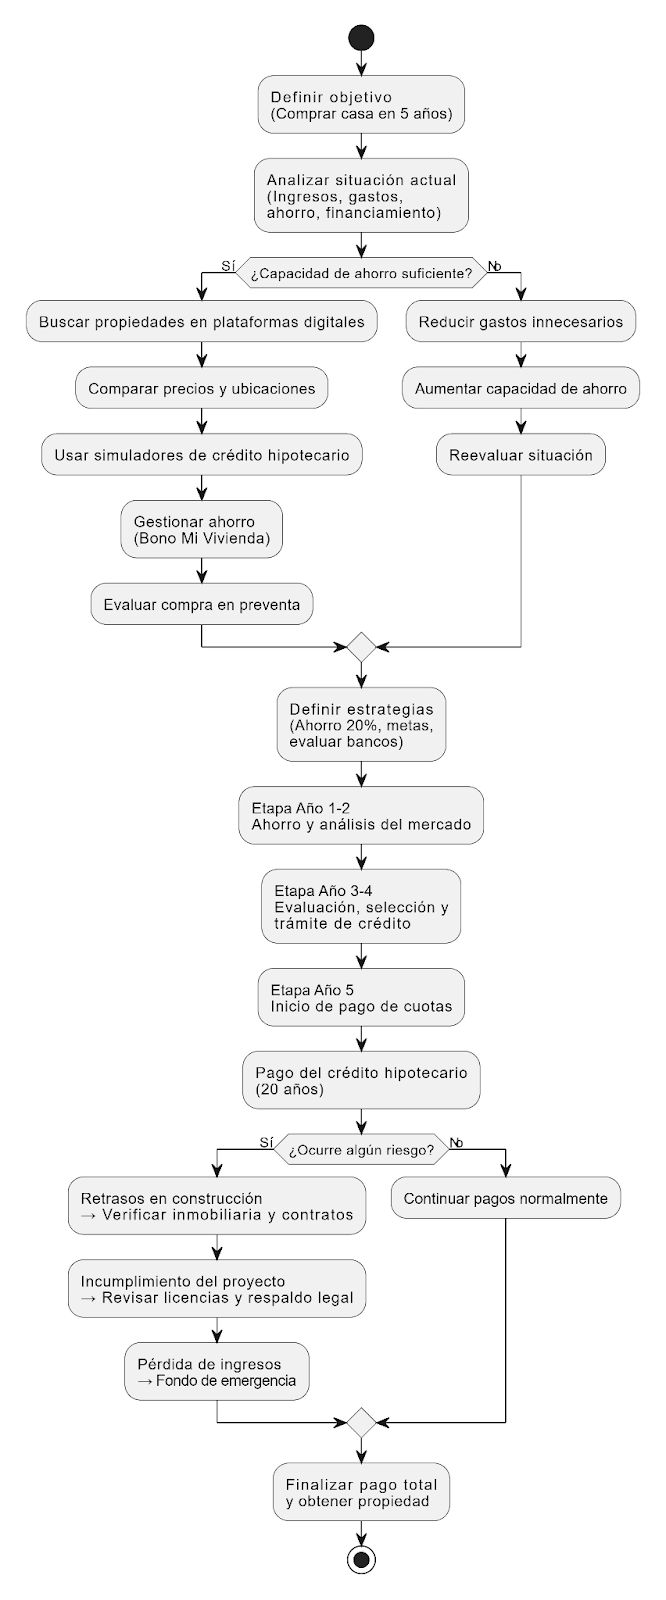
\includegraphics[height=0.8\textheight]{./assets/diagrama.png}
\end{center}

\end{document}
